\chapter{\textit{OwnCloud} пројекат}
\label{chap:ownCloud}
Рачунарство у облаку представља скуп ресурса, чији је задатак да омогући складиштење велике количине података или извршавање великог броја процеса. Основна карактеристика рачунарства у облаку је та да корисницима омогућава коришћење удаљених ресурса, при чему им није дозвољен физички приступ датим ресурсима. Пораст броја корисника са оваквим захтевима утицао је и на појаву великог броја комерцијалних платформи које нуде услугу рачунаарства у облаку, међу којима су \textit{Amazon}, \textit{Microsoft}, \textit{Dropbox} и многе друге. Једно од таквих решења је и \textit{ownCloud}\cite{owncloud} пројекат. 

На почетку основна идеја \textit{OwnCloud} пројекта је била да се обичном кориснику омогући да има приватно складиште на којем ће моћи да складишти своје податке. У међувремену, овај пројекат је добио много унапређења која нису директно везана за само складиштење података. Творац пројекта  Франк Карличек је идеју о потреби решења са "отвореним" лиценцама изнео на скупу програмера и успео је да обезбеди неопходан број учесника који ће допринети развоју и популаризацији овог пројекта.

\begin{figure}[H]
	\centering
	
\includegraphics[scale=0.4]{slike/owncloud_logo.png}
	\caption{\texttt{OwnCloud} лого}
\end{figure}

Постоје три могућности за приступ подацима на \textit{ownCloud-u}:
\begin{itemize}
	\item{Десктоп апликација - омогућава кориснику да складишти и/или преузима податке са удаљених ресурса},
	\item{\textit{WebDAV} технологија - погоднија од десктоп апликације, која се мора инсталирати на сваком рачунару, али са друге стране ограничава корисницима приступ само до података},
	\item{Веб апликација - нема ограничења као друге две опције. Дакле, омогућен је приступ свим погодностима које \textit{ownCloud} портал нуди и које ће бити представљне у наставку}.
\end{itemize}

\begin{figure}[H]
	\centering
	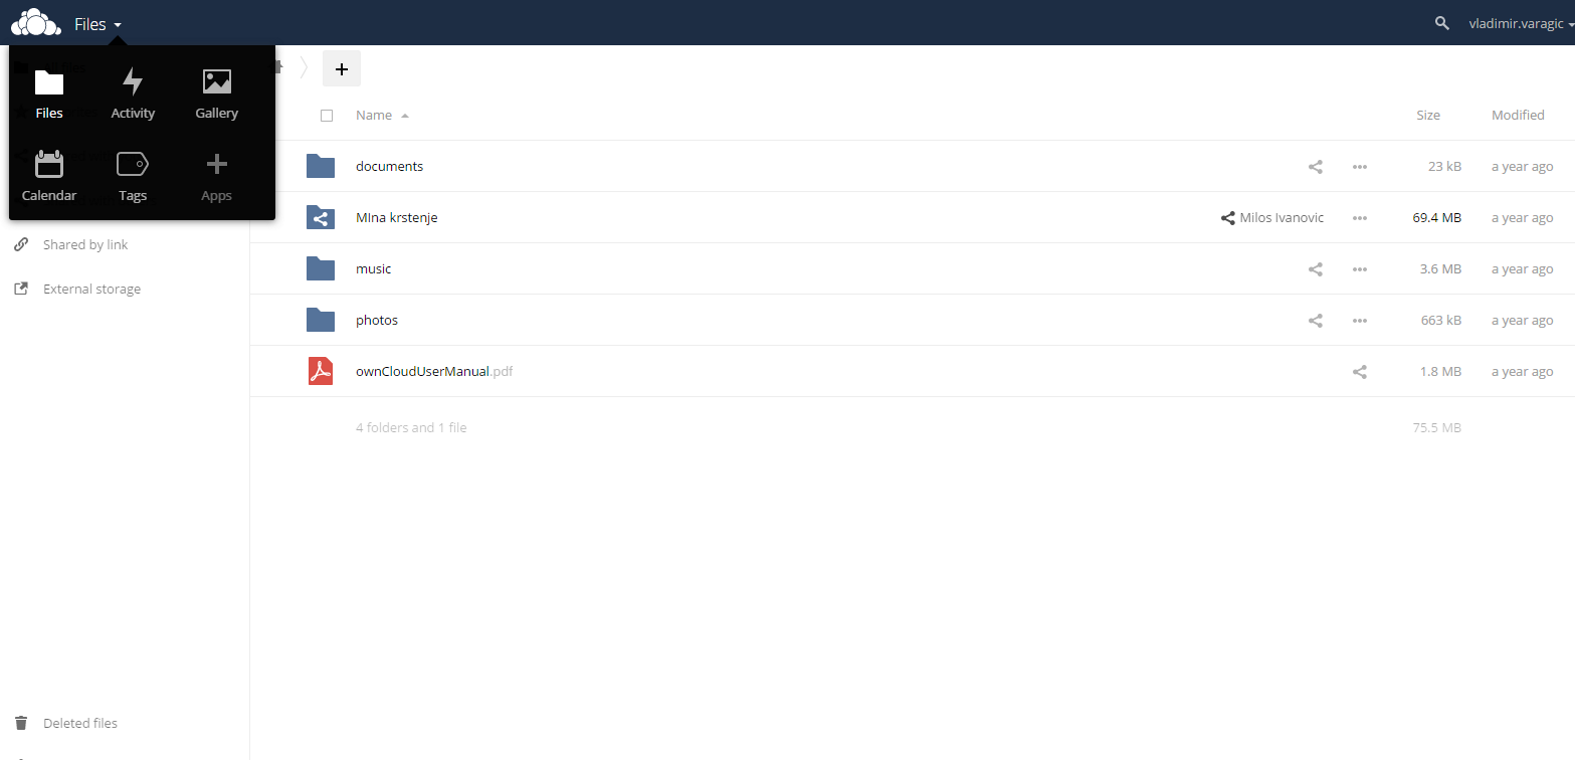
\includegraphics[scale=0.4]{slike/owncloud_ui_1.png}
	\caption{Кориснички интерфејс \textit{ownCloud} веб апликације}
	\label{fig:owncloud_ui_1}
\end{figure}

Као што се може видети на Слици \ref{fig:owncloud_ui_1}, неке од основних функционалности су:
\begin{itemize}
	\item Приказ листе фајлова и директоријума тренутно пријављеног корисника,
	\item Могућност додавања нових садржаја,
	\item Могућност брзе претраге садржаја,
	\item Листа доступних апликација,
	\item Могућност приступа приватним подацима корисника, као и могућност одјаве.
\end{itemize}

Поред могућности складиштења и приступа подацима \textit{ownCloud} веб апликација нуди могућност коришћења њених подапликација:
\begin{itemize}
	\item Вођење листе контаката,
	\item Дељење корисничких података између корисника истог складишта,
	\item Праћење активности корисника,
	\item Листа доступних апликација,
	\item Праћење календара, итд.
\end{itemize}

Посебна пажња биће посвећена \textit{Calendar} подапликацији.

\section{\textit{Calendar} подапликација}

Као што је већ раније поменуто, основна идеја и функција \textit{ownCloud} апликације је била да омогући складиштење података корисника, што није било довољно атрактивно. Увођењем платформе за креирање нових сервиса (подапликација) овај проблем је превазиђен. Један од њих је и \textit{Calendar} подапликација.

\begin{figure}[H]
	\centering
	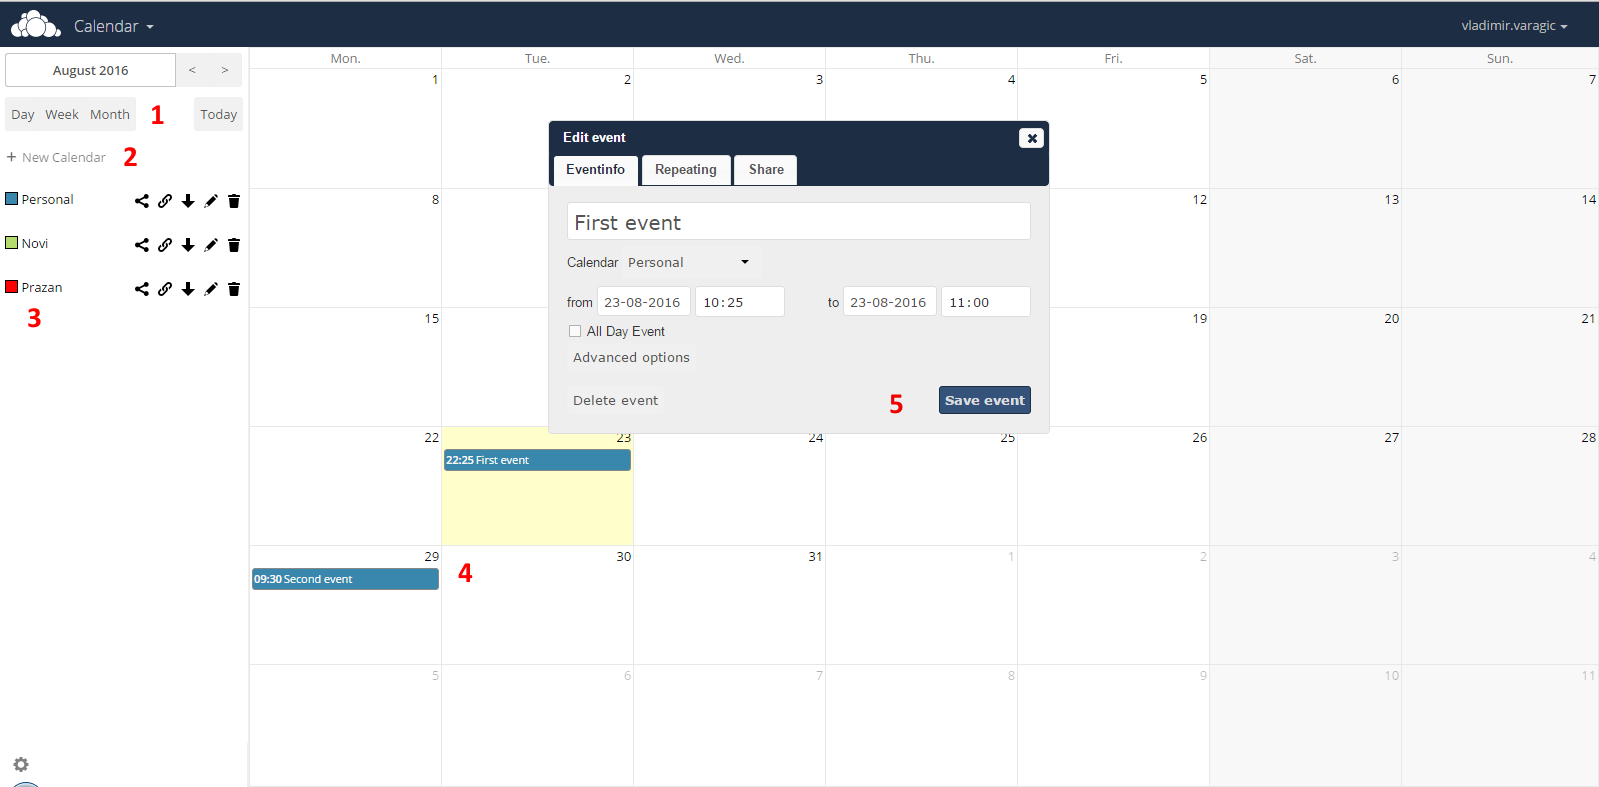
\includegraphics[scale=0.4]{slike/ownCloudCalendarDetails.png}
	\caption{Кориснички интерфејс \textit{ownCloud Calendar} подапликације}
	\label{fig:own_cloud_calendar_details}
\end{figure}

На Слици \ref{fig:own_cloud_calendar_details} су приказане све њене функционалности:
\begin{enumerate}
	\item Начин приказа календара (дневни, недељни, месечни),
	\item Креирање новог календара,
	\item Приказ постојећих календара,
	\item Приказ постојећих догађаја,
	\item Администрација (унос, измена, брисање) догађаја.
\end{enumerate}

Подапликација \textit{Calendar} је прилично једноставна и интуитивна за коришћење.